% (c)~2014 Claudio Carboncini - claudio.carboncini@gmail.com
% (c)~2014 Dimitrios Vrettos - d.vrettos@gmail.com
\chapter{Equazioni e disequazioni con moduli}

\section{Valore assoluto}
Riprendiamo la definizione già vista in ``Algebra~1'' di valore assoluto. Il \emph{valore assoluto} o \emph{modulo} di un numero $a$, indicato con $|a|$, è lo stesso numero $a$ se esso è maggiore o uguale a zero, o il suo opposto, cioè $-a$, se è minore di zero. In sintesi scriviamo:

\begin{equation*}
\left|a\right|=\begin{cases}a & \text{ se~~}a\ge 0\\
-a & \text{ se~~}a<0\end{cases}
\end{equation*}

Per esempio $\left|+7\right|=7$,~~$\left|-3\right|=-(-3)=3$,~~$\left|0\right|=0$,~~$\left|-1\right|=1$,~~$\left|1\right|=1$.

In maniera analoga definiamo il valore assoluto di un'espressione algebrica.
Il valore assoluto o modulo dell'espressione algebrica $E=x^2-3x$, indicato con $\left|x^2-3x\right|$, è una funzione definita per casi, cioè definita da espressioni diverse su sottoinsiemi diversi del dominio, 
\[f(x)=\left|x^2-3x\right|=\begin{cases}x^2-3x & \text{ se~~}x^2-3x\ge 0\\-\left(x^2-3x\right) & \text{ se~~}x^2-3x<0\end{cases}.\]
Risolvendo la disequazione $x^2-3x\ge 0$ si esplicitano i due sottoinsiemi in cui sono definite le due espressioni algebriche, cioè 
\[f(x)=\left|x^2-3x\right|=\begin{cases}x^2-3x & \text{ se~~}x\le 0\vee x\ge 3\\-x^2+3x & \text{ se~~}0<x<3\end{cases}.\]

In generale, la funzione \emph{valore assoluto} o \emph{modulo} di un'espressione algebrica viene definita come: 
\[\left|f(x)\right|=\begin{cases}f(x) & \text{ se~~}f(x)\ge 0\\-f(x) & \text{ se~~}f(x)<0\end{cases}.\]

La funzione $f(x)$ è detta \textit{argomento del valore assoluto}.

\begin{exrig}
\begin{esempio}
Per la funzione $f(x)=\left|\sqrt 3+3x\right|$ trovare le espressioni algebriche che descrivono i due casi.

Per definizione si ha: 
\[f(x)=\left|\sqrt 3+3x\right|=\begin{cases}\sqrt 3+3x & \text{ se~~}\sqrt 3+3x\ge 0\:\Rightarrow\: x\ge -\dfrac{\sqrt 3} 3\\-\sqrt 3-3x & \text{ se~~}\sqrt 3+3x<0\:\Rightarrow\: x<-\dfrac{\sqrt 3} 3\end{cases}.\]
\end{esempio}
\pagebreak
\begin{esempio}
Data la funzione $f(x)=\left|x^2-4\right|+\left|x+1\right|-2x$ descriverla per casi, eliminando i valori assoluti.

Dobbiamo studiare i segni dei due binomi in valore assoluto 
\[\begin{array}{l}x^2-4\ge 0\quad\Rightarrow\quad x\le -2\vee x\ge 2~\text{ e} \\x+1\ge 0\quad\Rightarrow\quad x\ge -1.\end{array}\]

%\[x^2-4\ge 0\quad\Rightarrow\quad x\le -2\vee x\ge 2\] e \[x+1\ge 0\quad\Rightarrow\quad x>-1.\] 
La situazione è rappresentata con maggiore chiarezza nel grafico seguente.
\begin{center}
% (c) 2013 Claudio Carboncini - claudio.carboncini@gmail.com
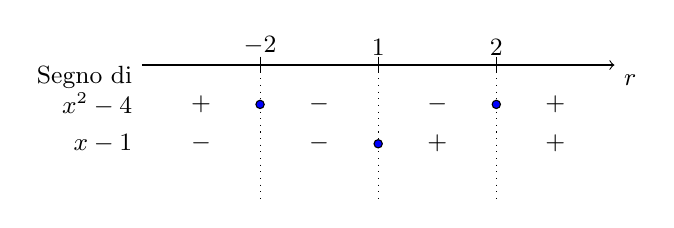
\begin{tikzpicture}[font=\small,x=10mm, y=10mm]

\draw[->] (0,0) -- (6,0) node [below right] () {$r$};

\foreach \x in {1.5,3,4.5}{
\draw(\x,3pt)--(\x,-3pt);
\begin{scope}[dotted]
\draw (\x,0) -- (\x,-1.7);
\end{scope}}

\node[left] at (0,-0.15) {Segno di};
\node[left] at (0,-0.5) {$x^2-4$};
\node[left] at (0,-1) {$x-1$};
\node[above]  at (1.5,0) {$-2$};
\node[above]  at (3,0) {$1$};
\node[above]  at (4.5,0) {$2$};
\node[] at (.75,-0.5) {$+$};
\node[] at (2.25,-0.5) {$-$};
\node[] at (3.75,-0.5) {$-$};
\node[] at (5.25,-0.5) {$+$};
\node[] at (.75,-1) {$-$};
\node[] at (2.25,-1) {$-$};
\node[] at (3.75,-1) {$+$};
\node[] at (5.25,-1) {$+$};
\draw[fill=blue] (3,-1)circle (1.5pt);
\draw[fill=blue] (1.5,-.5)circle (1.5pt);
\draw[fill=blue] (4.5,-.5)circle (1.5pt);
\end{tikzpicture}

\end{center}

\begin{itemize*}
\item Nell'intervallo $x\le -2$ l'argomento del primo valore assoluto è positivo o uguale a 0 per $x=-2$ e quello del secondo è negativo;
\item nell'intervallo $-2<x<-1$ tutti e due gli argomenti del valore assoluto sono negativi;
\item nell'intervallo $-1\le x\le 2$ l'argomento del primo valore assoluto è negativo o uguale a 0 per $x=2$, quello del secondo è positivo o uguale a 0 per $x=1$;
\item nell'intervallo $x>2$ entrambi gli argomenti sono positivi.
\end{itemize*}
In sintesi 
\[f(x)=
\begin{cases}(x^2-4)-(x+1)-2 & \text{ se~~}x\le -2 \\
-(x^2-4)-(x+1)-2x & \text{ se~~}-2<x<-1 \\
-(x^2-4)+(x+1)-2x & \text{ se~~}-1\le x\le 2 \\
(x^2-4)+(x+1)-2x & \text{ se~~}x>2
\end{cases}.\]
\end{esempio}
\end{exrig}
\ovalbox{\risolvii \ref{ese:7.1}, \ref{ese:7.2}, \ref{ese:7.3}}

\section{Equazioni in una incognita in valore assoluto}
\subsection{Equazioni nelle quali l'incognita è presente solo all'interno del modulo}
\begin{itemize}
\item Equazioni con valore assoluto del tipo $\left|f(x)\right|=k\text{ con }k\ge 0$.
\end{itemize}

\begin{exrig}
\begin{esempio}\label{es:7.3}
Risolvere la seguente equazione $\left|x^2-7\right|=3$.

Per la definizione di valore assoluto si ha che
$\left|x^2-7\right|=\begin{cases}
x^2-7 & \text{ se~~}x^2-7 \ge 0\\
-x^2+7 & \text{ se~~}x^2-7 < 0\\
\end{cases}\;$, pertanto l'equazione diventa

\[\left|x^2-7\right|=3 \:\Rightarrow \begin{cases}
x^2-7=3 & \text{ se~~}x^2-7 \ge 0\\
-x^2+7=3 & \text{ se~~}x^2-7 < 0\\
\end{cases}\]
ovvero il tutto equivale all'unione dei due sistemi

\[\left\{\begin{array}{l}{x^2-7\ge 0}\\{x^2-7=3}\end{array}\right.\cup \left\{\begin{array}{l}{x^2-7<0}\\{-x^2+7=3}\end{array}\right..\]

Moltiplicando per $-1$ ambo i membri dell'equazione del secondo sistema otteniamo: \[\left\{\begin{array}{l}{x^2-7\ge 0}\\{x^2-7=3}\end{array}\right.\cup \left\{\begin{array}{l}{x^2-7<0}\\{x^2-7=-3}\end{array}\right..\]

Si vede abbastanza facilmente che sia nel primo che nel secondo sistema le due disequazioni sono sempre verificate. Infatti, nel primo sistema l'equazione $x^2-7=3$ verifica automaticamente la disequazione $x^2-7\ge 0$ in quanto è richiesto che $x^2-7$ sia uguale a $3$, pertanto è necessariamente positivo.
Stesso ragionamento vale per il secondo sistema. In altre parole, per risolvere la disequazione data è sufficiente risolvere le due equazioni $x^2-7=3$ e $x^2-7=-3$ unendone le soluzioni. Quindi
\[\begin{array}{l}x^2-7=3\:\Rightarrow\: x^2=10\:\Rightarrow\: x_1=-\sqrt{10}\;\vee\; x_2=\sqrt{10}~\text{ e} \\x^2-7=-3\:\Rightarrow\: x^2=4\:\Rightarrow\: x_3=-2\;\vee\; x_4=2.\end{array}\]

L'insieme delle soluzioni è quindi: $\left\{-\sqrt{10}\text{, }\sqrt{10}\text{, }-2\text{, }+2\right\}$.
\end{esempio}
\end{exrig}

\paragraph{Procedura risolutiva} Per risolvere un'equazione del tipo $\left|f(x)\right|=k\,\text{ con }k\ge 0$ è sufficiente risolvere la doppia equazione $f(x)=\pm k$.
\begin{exrig}
\begin{esempio}
Risolvere la seguente equazione $\left|x^2-x\right|=1$.

L'equazione $\left|x^2-x\right|=1$ si risolve unendo le soluzioni delle equazioni $x^2-x=1$ e $x^2-x=-1$. cioè:
\[\begin{array}{l}x^2-x=1\quad\Rightarrow\quad x^2-x-1=0\quad\Rightarrow\quad x_1=\dfrac{1-\sqrt 5} 2\;\vee\; x_2=\dfrac{1+\sqrt 5} 2~\text{ e} \\x^2-x=-1\quad\Rightarrow\quad x^2-x+1=0\quad\Rightarrow\quad \Delta <0\quad\Rightarrow\quad\IS=\emptyset.\end{array}\]

L'insieme soluzione dell'equazione data è quindi \[\IS=\left\{\dfrac{1-\sqrt 5} 2\text{, }\dfrac{1+\sqrt 5} 2\right\}.\]
\end{esempio}
\end{exrig}

\begin{itemize}
\item Equazioni con valore assoluto del tipo ${\left|f(x)\right|=k\text{ con }k<0}$.
\end{itemize}

Se $k<0$ l'equazione è impossibile. In questo caso $\left|f(x)\right|=k$ è una contraddizione, in quanto un valore assoluto di una espressione è sempre un valore positivo.

\begin{exrig}
\begin{esempio}
Risolvere la seguente equazione $\left|x-7\right|=-1$.
Impostiamo la ricerca delle soluzioni con il metodo generale presentato nell'esempio~\ref{es:7.3}. L'equazione corrisponde alla soluzione dell'unione dei due sistemi seguenti
\[\left\{\begin{array}{l}{x-7\ge 0}\\{x-7=-1}\end{array}\right. \cup~ \left\{\begin{array}{l}{x-7<0}\\{x-7=1}\end{array}\right..\]
Entrambi i sistemi non hanno soluzioni reali. L'equazione è impossibile.
\end{esempio}
\end{exrig}
\ovalbox{\risolvii \ref{ese:7.3}, \ref{ese:7.4}, \ref{ese:7.5}, \ref{ese:7.6}, \ref{ese:7.7}}

\subsection{Equazioni nelle quali l'incognita si trova anche fuori dal modulo}
\begin{exrig}
\begin{esempio}
Risolvere la seguente equazione $\left|-1+3x\right|=7x+4$.

L'equazione presenta un valore assoluto al primo membro.

Tenendo conto che 
\[\left|-1+3x\right|=\spazielenx{\begin{cases}-1+3x & \text{ se~~}-1+3x\ge 0\:\Rightarrow\: x\ge \frac 1 3\\1-3x & \text{ se~~}-1+3x<0\:\Rightarrow\: x<\frac 1 3\end{cases}\text{,}}\]
l'equazione si trasforma nell'unione dei due sistemi 
\[\left\{\begin{array}{l}{x\ge \dfrac 1 3}\\{-1+3x=7x+4}\end{array}\right.\cup \left\{\begin{array}{l}{x<\dfrac 1 3}\\{1-3x=7x+4}\end{array}\right..\]

Risolvendo si ha 
\[\left\{\begin{array}{l}{x\ge \dfrac 1 3}\\{4x=-5\:\Rightarrow\: x=-\dfrac 5 4}\end{array}\right.\cup \left\{\begin{array}{l}{x<\dfrac 1 3}\\{10x=-3\:\Rightarrow\: x=-\dfrac 3{10}}\end{array}\right..\]

La soluzione $-\dfrac 5 4$ non è accettabile in quanto non è maggiore di $\dfrac 1 3$. Pertanto rimane la soluzione $x=-\dfrac 3{10}$ (che è minore di $\dfrac{1}{3}$).
\end{esempio}

\begin{esempio}
Risolvere la seguente equazione $\left|-2x+5\right|=x-3$.

Esplicitiamo i due casi dell'argomento 
\[\left|-2x+5\right|=\begin{cases}-2x+5 & \text{ se~~}-2x+5\ge 0\:\Rightarrow\: x\le \dfrac 5 2\\2x-5 & \text{ se~~}-2x+5<0\:\Rightarrow\: x>\dfrac 5 2\end{cases}.\]
L'equazione si trasforma quindi nell'unione dei due sistemi:
\[\left\{\begin{array}{l}{x\le \dfrac 5 2}\\{-2x+5=x-3}\end{array}\right.\cup \left\{\begin{array}{l}{x>\dfrac 5 2}\\{2x-5=x-3}\end{array}\right..\]

Risolviamo ciascun sistema 
\[\left\{\begin{array}{l}{x\le \dfrac 5 2}\\{-3x=-8\:\Rightarrow\: x=\dfrac 8 3}\end{array}\right.\cup \left\{\begin{array}{l}{x>\dfrac 5 2}\\{x=2}\end{array}\right.\] 
ognuno dei quali risulta impossibile, cioè $\IS_1=\emptyset$ e $\IS_2=\emptyset $.

Quindi l'insieme soluzione dell'equazione data è $\IS=\IS_1\cup \IS_2=\emptyset \cup \emptyset =\emptyset $: l'equazione è impossibile.
\end{esempio}

\begin{esempio}
Risolvere la seguente equazione $\left|2x-1\right|=x+2$.

L'equazione si trasforma nell'unione dei due sistemi 
\[ \left\{\begin{array}{l}{2x-1\ge 0}\\{2x-1=x+2}\end{array}\right.\cup \left\{\begin{array}{l}{2x-1<0}\\{-2x+1=x+2}\end{array}\right.\Rightarrow
\left\{\begin{array}{l}{x\ge \dfrac 1 2}\\{x=3}\end{array}\right.\cup \left\{\begin{array}{l}{x<\dfrac 1 2}\\{x=-\dfrac 1 2}\end{array}\right..\] 
Quindi le soluzioni sono $x=3$~~e~~$x=-\dfrac 1 2$.
\end{esempio}
\end{exrig}
\ovalbox{\risolvii \ref{ese:7.8}, \ref{ese:7.9}, \ref{ese:7.10}, \ref{ese:7.11}, \ref{ese:7.12}, \ref{ese:7.13}, \ref{ese:7.14}, \ref{ese:7.15}, \ref{ese:7.16}}

\section{Equazioni con più espressioni in valore assoluto}

\begin{exrig}
\begin{esempio}
Risolvere la seguente equazione $\left|2x-3\right|-\left|1-2x\right|+x=4$.

L'equazione presenta due espressioni in valore assoluto; ciascuna espressione sarà sviluppata in due modi diversi dipendenti dal segno assunto dai rispettivi argomenti. Si presenteranno allora quattro casi e l'insieme soluzione dell'equazione sarà ottenuto dall'unione delle soluzioni dei singoli casi. Per semplificare il procedimento studiamo il segno di ciascun argomento e poi confrontiamo i segni con uno schema grafico:
\begin{center}
% (c) 2013 Claudio Carboncini - claudio.carboncini@gmail.com
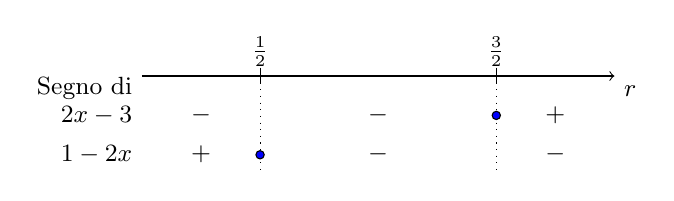
\begin{tikzpicture}[font=\small,x=10mm, y=10mm]

\draw[->] (0,0) -- (6,0) node [below right] () {$r$};

\foreach \x in {1.5,4.5}{
\draw(\x,3pt)--(\x,-3pt);
\begin{scope}[dotted]
\draw (\x,0) -- (\x,-1.2);
\end{scope}}

\node[left] at (0,-0.15) {Segno di};
\node[left] at (0,-0.5) {$2x-3$};
\node[left] at (0,-1) {$1-2x$};
\node[above]  at (1.5,0) {$\frac 1 2$};
\node[above]  at (4.5,0) {$\frac 3 2$};
\node[] at (.75,-0.5) {$-$};
\node[] at (3,-0.5) {$-$};
\node[] at (5.25,-0.5) {$+$};
\node[] at (.75,-1) {$+$};
\node[] at (3,-1) {$-$};
\node[] at (5.25,-1) {$-$};
\draw[fill=blue] (1.5,-1)circle (1.5pt);
\draw[fill=blue] (4.5,-.5)circle (1.5pt);

\end{tikzpicture}

\end{center}
Si presentano tre casi:
\begin{itemize*}
\item Caso I: $ \left\{\begin{array}{l}{x< \frac 1 2}\\{-(2x-3)-(1-2x)+x=4}\end{array}\right. $;
\item Caso II: $ \left\{\begin{array}{l}{\frac 1 2\le x<\frac 3 2}\\{-(2x-3)+(1-2x)+x=4}\end{array}\right. $;
\item Caso III: $ \left\{\begin{array}{l}{x\ge \frac 3 2}\\{(2x-3)+(1-2x)+x=4}\end{array}\right. $.
\end{itemize*}
In ogni sistema la prima condizione è la disequazione che vincola il segno degli argomenti e la seconda è l'equazione che risulta in base al segno definito. Risolviamo.

Caso I:
\[\left\{\begin{array}{l}x< \frac 1 2\\-(2x-3)-(1-2x)+x=4\end{array}\right.\Rightarrow \left\{\begin{array}{l}x< \frac 1 2\\x=2\end{array}\right.\Rightarrow\: \IS_1=\emptyset .\]
Il sistema è impossibile in quanto $2$ non è minore di $\frac 1 2$.

Caso II: 
\[\left\{\begin{array}{l}\frac 1 2\le x< \frac 3 2\\-(2x-3)+(1-2x)+x=4\end{array}\right.\Rightarrow \left\{\begin{array}{l}\frac 1 2\le x< \frac 3 2\\x=0\end{array}\right.\Rightarrow\: \IS_2=\emptyset .\]
Il sistema è impossibile in quanto 0 non appartiene all'intervallo $\left[\dfrac{1}{2}\text{, }\dfrac{3}{2}\right)$.

Caso III: 
\[\left\{\begin{array}{l}x\ge\frac 3 2\\(2x-3)+(1-2x)+x=4\end{array}\right.\Rightarrow \left\{\begin{array}{l}x\ge\frac 3 2\\x=6\end{array}\right.\Rightarrow\: \IS_3=\{6\}.\]
La soluzione in questo caso è accettabile.

Conclusione: $\IS=\IS_1\cup \IS_2\cup \IS_3=\{6\}$.
\end{esempio}

\begin{esempio}
Risolvere la seguente equazione $\left|x^2-4\right|-3x=\left|x-1\right|$.

Confrontiamo il segno di ciascun argomento servendoci dello schema:
\begin{center}
% (c) 2013 Claudio Carboncini - claudio.carboncini@gmail.com
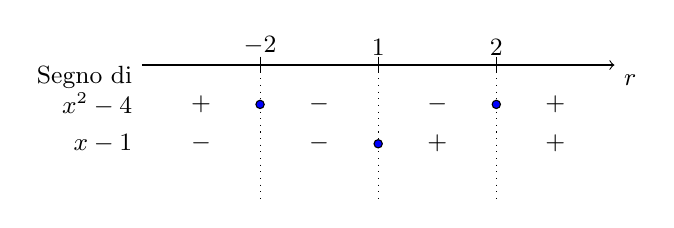
\begin{tikzpicture}[font=\small,x=10mm, y=10mm]

\draw[->] (0,0) -- (6,0) node [below right] () {$r$};

\foreach \x in {1.5,3,4.5}{
\draw(\x,3pt)--(\x,-3pt);
\begin{scope}[dotted]
\draw (\x,0) -- (\x,-1.7);
\end{scope}}

\node[left] at (0,-0.15) {Segno di};
\node[left] at (0,-0.5) {$x^2-4$};
\node[left] at (0,-1) {$x-1$};
\node[above]  at (1.5,0) {$-2$};
\node[above]  at (3,0) {$1$};
\node[above]  at (4.5,0) {$2$};
\node[] at (.75,-0.5) {$+$};
\node[] at (2.25,-0.5) {$-$};
\node[] at (3.75,-0.5) {$-$};
\node[] at (5.25,-0.5) {$+$};
\node[] at (.75,-1) {$-$};
\node[] at (2.25,-1) {$-$};
\node[] at (3.75,-1) {$+$};
\node[] at (5.25,-1) {$+$};
\draw[fill=blue] (3,-1)circle (1.5pt);
\draw[fill=blue] (1.5,-.5)circle (1.5pt);
\draw[fill=blue] (4.5,-.5)circle (1.5pt);
\end{tikzpicture}

\end{center}
In questo esempio dobbiamo esaminare 4 casi che si esplicitano nei sistemi:
\begin{itemize*}
\item Caso I: 
\[\left\{\begin{array}{l}{x< -2}\\{x^2-4-3x=-x+1}\:\Rightarrow\: x_1=1-\sqrt 6\;\vee\; x_2=1+\sqrt 6\end{array}\right.\Rightarrow\: \IS_1=\emptyset .\]
\item Caso II: 
\[\left\{\begin{array}{l}{-2\le x<1}\\{-x^2+4-3x=-x+1}\:\Rightarrow\: x_1=-3\;\vee\; x_2=1\end{array}\right.\Rightarrow\: \IS_2=\emptyset .\]
\item Caso III: 
\[\left\{\begin{array}{l}{1\le x<2}\\{-x^2+4-3x=x-1}\:\Rightarrow\: x_1=-5\;\vee\; x_2=1\end{array}\right.\Rightarrow\: \IS_3=\{1\}.\]
\item Caso IV: 
\[\left\{\begin{array}{l}{x\ge 2}\\{x^2-4-3x=x-1}\:\Rightarrow\: x_1=2-\sqrt 7\;\vee\; x_2=2+\sqrt 7\end{array}\right.\Rightarrow\: \IS_4=\left\{2+\sqrt 7\right\}.\]
\end{itemize*}

Conclusione: $\IS=\IS_1\cup \IS_2\cup \IS_3\cup \IS_4=\left\{1\text{, }2+\sqrt 7\right\}$.
\end{esempio}
\end{exrig}

\begin{procedura} {Risoluzione di un'equazione con valori assoluti:}
\begin{enumeratea}
\item \emph{l'incognita è presente solo nell'argomento del modulo.} L'equazione è del tipo $\left|f(x)\right|=k$ e si risolve studiando $f(x)=\pm k$. Se $k<0$ l'equazione è impossibile;
\item \emph{l'incognita si trova anche al di fuori del modulo.} Si analizza il segno dell'argomento del modulo e si risolvono i due sistemi dove la prima condizione è la disequazione che vincola il segno dell'argomento e la seconda è l'equazione che risulta in base al segno definito. L'insieme soluzione dell'equazione è dato dall'unione degli insiemi soluzione dei due sistemi;
\item \emph{è presente più di un modulo che ha l'incognita nel proprio argomento.} Si studia il segno di ogni argomento e dallo schema che ne segue si costruiscono e quindi si risolvono i sistemi in cui la prima condizione è la disequazione che vincola il segno degli argomenti e la seconda è l'equazione in base al segno definito. Anche in questo caso l'insieme soluzione dell'equazione è dato dall'unione degli insiemi soluzione dei vari sistemi.
\end{enumeratea}
\end{procedura}
\ovalbox{\risolvii \ref{ese:7.17}, \ref{ese:7.18}, \ref{ese:7.19}, \ref{ese:7.20}, \ref{ese:7.21}, \ref{ese:7.22}, \ref{ese:7.23}, \ref{ese:7.24}, \ref{ese:7.25}, \ref{ese:7.26}, \ref{ese:7.27}, \ref{ese:7.28}, \ref{ese:7.29}, \ref{ese:7.30}}

\section{Disequazioni con valore assoluto}
Le disequazioni con i moduli si risolvono in modo analogo alle equazioni con moduli.

\subsection{Disequazioni in cui l'incognita si trova solo nel modulo}

\begin{itemize}
\item Disequazioni con valore assoluto nella forma $\left|f(x)\right|<k \text{ con }  k>0 $.
\end{itemize}

La disequazione si risolve studiando l'unione dei due sistemi 
\[\left\{\begin{array}{l}{f(x)\ge 0}\\{f(x)<k}\end{array}\right.\cup\left\{\begin{array}{l}{f(x)< 0}\\{f(x)>-k}\end{array}\right.\]
che hanno soluzioni $ 0\le f(x)<k\;\vee\; -k<f(x)<0 $ cioè:
\[-k<f(x)<k\quad \text{ o anche }\quad\left\{\begin{array}{l}{f(x)< k}\\{f(x)>-k}\end{array}\right..\]

\begin{exrig}
\begin{esempio}
Risolvere la seguente disequazione $\left|x^2-1\right|<3$.

La disequazione diventa $-3<x^2-1<3$ oppure 
\[\left\{\begin{array}{l}{x^2-1<3}\\{x^2-1>-3}\end{array}\right.\Rightarrow \left\{\begin{array}{l}{x^2<4}\\{x^2>-2}\end{array}\right..\]

La prima disequazione $x^2<4$ è verificata per $-2<x<2$.

La seconda è sempre verificata perché il quadrato $x^2$ è sempre maggiore di un numero negativo.
L'insieme soluzione della disequazione assegnata è quindi $-2<x<2$.

\end{esempio}
\end{exrig}

\begin{itemize}
\item Disequazioni con valore assoluto nella forma $\left|f(x)\right|>k \text{ con } k>0 $.
\end{itemize}

La disequazione si risolve studiando l'unione dei due sistemi 
\[\left\{\begin{array}{l}{f(x)\ge 0}\\{f(x)>k}\end{array}\right.\cup\left\{\begin{array}{l}{f(x)< 0}\\{f(x)<-k}\end{array}\right.\]
che hanno soluzioni \[ f(x)<-k\;\vee\; f(x)>k. \]

%\paragraph{Secondo caso:} disequazioni nella forma $\left|f(x)\right|>k$ con $ k>0 $.

%Per il procedimento svolto nel caso precedente queste disequazioni si trasformano sempre nelle disequazioni \[ f(x)<-k\;\vee\; f(x)>k. \]

\begin{exrig}
\begin{esempio}
Risolvere la seguente equazione $\left|x^2-4\right|>4$.

L'equazione diventa $x^2-4<-4\;\vee\; x^2-4>4$. Spostando $-4$ al secondo membro otteniamo $x^2<0\;\vee\; x^2>8$.

La prima disequazione $x^2<0$ non ha soluzioni in quanto il quadrato $x^2$ non può essere minore di 0.
La seconda ha per soluzioni $x<-2\sqrt 2\;\vee\; x>2\sqrt 2$.
\end{esempio}
\end{exrig}

\subsection{Disequazioni in cui l'incognita si trova anche fuori dal modulo}

\begin{exrig}
\begin{esempio}
Risolvere la seguente disequazione $\left|x^2-x\right|<2x^2+3x-1$.

Studiamo il segno dell'argomento del modulo 
\[x^2-x\ge 0 \quad\Rightarrow\quad x(x-1)\ge 0 \quad\Rightarrow\quad x\le 0\vee x\ge 1.\]

La disequazione assegnata si sdoppia nell'unione di due sistemi:

\[\left\{\begin{array}{l}{x\le 0\;\vee\; x\ge 1}\\{x^2-x<2x^2+3x-1}\end{array}\right.\cup \left\{\begin{array}{l}{0<x<1}\\{-x^2+x<2x^2+3x-1}\end{array}\right..\]

 Semplificando le disequazioni si ha:
\begin{equation*}
\left\{\begin{array}{l}{x\le 0\;\vee\; x\ge 1}\\{x^2+4x-1>0}\end{array}\right.\cup \left\{\begin{array}{l}{0<x<1}\\{3x^2+2x-1>0}\end{array}\right..
\end{equation*}

Quindi rappresentiamo gli insiemi soluzione dei due sistemi in uno schema, così possiamo trovare agevolmente l'insieme soluzione della disequazione data.

\begin{center}
% (c) 2013 Claudio Carboncini - claudio.carboncini@gmail.com
\begin{tikzpicture}[font=\small,x=10mm, y=10mm]

%IS1
\draw[->] (0,0) -- (8,0) node [below right] () {$r$};

\foreach \x in {1.5,3.5,4.5,6.5}{
\draw(\x,2pt)--(\x,-2pt);
\draw[dotted] (\x,0) -- (\x,-2);
}
\begin{scope}[dotted]
\draw (3.5,-.5) -- (6.5,-.5);
\draw (1.5,-1) -- (5,-1);
\draw (0,-1.5) -- (8,-1.5);
\end{scope}

\node[above]  at (1.5,0) {$-2- \sqrt{5}$};
\node[above]  at (3.5,0) {$0$};
\node[above]  at (4.5,0) {$-2+ \sqrt{5}$};
\node[above]  at (6.5,0) {$1$};
\pattern[pattern= north east lines, pattern color=red] (0,-2) rectangle (1.5,-1.5);
\pattern[pattern= north east lines, pattern color=red] (6.5,-2) rectangle (8,-1.5);

\node[left] () at (-0.2,-.5) {$x^2-x\ge0$};
\node[left] () at (-0.2,-1) {$x^2+4x-1>0$};
\node[left] () at (-0.2,-1.75) {$\IS_{1}$};

\begin{scope}[blue,thick]
\draw (0,-.5) -- (3.5,-.5);
\draw (6.5,-.5) -- (8,-.5);
\draw (0,-1) -- (1.5,-1);
\draw (4.5,-1) -- (8,-1);
\draw (0,-1.5) -- (1.5,-1.5);
\draw (6.5,-1.5) -- (8,-1.5);

\draw[fill=blue] (3.5,-.5)circle (1.5pt);
\draw[fill=blue] (6.5,-.5)circle (1.5pt);
\draw[fill=white] (1.5,-1)circle (1.5pt);
\draw[fill=white] (4.5,-1)circle (1.5pt);
\draw[fill=white] (1.5,-1.5)circle (1.5pt);
\draw[fill=blue] (6.5,-1.5)circle (1.5pt);
\end{scope}

%IS2
\begin{scope}[shift={(0,-.25)}]
\draw[->] (0,-2.5) -- (8,-2.5) node [below right] () {$r$};

\begin{scope}[shift={(0,-2.5)}]
\foreach \x in {2,3.5,5,6.5}{
\draw(\x,2pt)--(\x,-2pt);
\draw[dotted] (\x,0) -- (\x,-2);
}
\end{scope}
\begin{scope}[dotted]
\draw (0,-3) -- (3.5,-3);
\draw (6.5,-3) -- (8,-3);
\draw (1.5,-3.5) -- (5,-3.5);
\draw (0,-4) -- (8,-4);
\end{scope}

\node[above]  at (2,-2.5) {$-1$};
\node[above]  at (3.5,-2.5) {$0$};
\node[above]  at (5,-2.5) {$\frac 1 3$};
\node[above]  at (6.5,-2.5) {$1$};
\pattern[pattern= north east lines, pattern color=red] (5,-4.5) rectangle (6.5,-4);

\node[left] () at (-0.2,-3) {$x^2-x<0$};
\node[left] () at (-0.2,-3.5) {$3x^2+2x-1>0$};
\node[left] () at (-0.2,-4.25) {$\IS_{2}$};

\begin{scope}[blue,thick]
\draw (3.5,-3) -- (6.5,-3);
\draw (0,-3.5) -- (2,-3.5);
\draw (5,-3.5) -- (8,-3.5);
\draw (5,-4) -- (6.5,-4);

\draw[fill=white] (3.5,-3)circle (1.5pt);
\draw[fill=white] (6.5,-3)circle (1.5pt);
\draw[fill=white] (2,-3.5)circle (1.5pt);
\draw[fill=white] (5,-3.5)circle (1.5pt);
\draw[fill=white] (5,-4)circle (1.5pt);
\draw[fill=white] (6.5,-4)circle (1.5pt);
\end{scope}
\end{scope}

%IS1 unito IS2
\begin{scope}[shift={(0,-.5)}]
\draw[->] (0,-5) -- (8,-5) node [below right] () {$r$};

\begin{scope}[shift={(0,-5)}]
\foreach \x in {1.5,5}{
\draw(\x,2pt)--(\x,-2pt);
\draw[dotted] (\x,0) -- (\x,-1);
}
\end{scope}
\node[above]  at (1.5,-5) {$-2- \sqrt{5}$};
\node[above]  at (5,-5) {$\frac 1 3$};
%\node[above]  at (6.5,-5) {$1$};
\node[left] () at (-0.2,-5.75) {$\IS_{1}\cup\IS_{2}$};
\pattern[pattern= north east lines, pattern color=Maroon] (0,-5.5) rectangle (1.5,-6);
\pattern[pattern= north east lines, pattern color=Maroon] (5,-5.5) rectangle (8,-6);
\draw[dotted] (0,-5.5) -- (8,-5.5);
\begin{scope}[blue,thick]
\draw (0,-5.5) -- (1.5,-5.5);
\draw (5,-5.5) -- (8,-5.5);
\draw[fill=white] (1.5,-5.5)circle (1.5pt);
\draw[fill=white] (5,-5.5)circle (1.5pt);
\end{scope}
\end{scope}

\end{tikzpicture}

\end{center}

L'insieme soluzione della disequazione data è $x<-2-\sqrt 5\;\vee\; x>\dfrac 1 3$.
\end{esempio}
\end{exrig}

\subsection{Disequazioni con più valori assoluti}
\begin{exrig}
\begin{esempio}
Risolvere la seguente disequazione $\left|x+1\right|\ge \left|x^2-1\right|$.

Studiamo il segno di ciascun argomento e poi confrontiamo i segni con uno schema grafico:
\begin{center}
% (c) 2013 Claudio Carboncini - claudio.carboncini@gmail.com
\begin{tikzpicture}[font=\small,x=10mm, y=10mm]

\draw[->] (0,0) -- (6,0) node [below right] () {$r$};

\foreach \x in {1.5,4.5}{
\draw(\x,3pt)--(\x,-3pt);
\begin{scope}[dotted]
\draw (\x,0) -- (\x,-1.7);
\end{scope}}

\node[left] at (0,-0.15) {Segno di};
\node[left] at (0,-0.5) {$x+1$};
\node[left] at (0,-1) {$x^2-1$};

\node[above]  at (1.5,0) {$-1$};
\node[above]  at (4.5,0) {$1$};

\node[] at (.75,-0.5) {$-$};
\node[] at (3,-0.5) {$+$};
\node[] at (5.25,-0.5) {$+$};

\node[] at (.75,-1) {$+$};
\node[] at (3,-1) {$-$};
\node[] at (5.25,-1) {$+$};

\draw[fill=blue] (1.5,-.5)circle (1.5pt);
\draw[fill=blue] (1.5,-1)circle (1.5pt);
\draw[fill=blue] (4.5,-1)circle (1.5pt);

\end{tikzpicture}

\end{center}
Si presentano tre casi, quindi tre sistemi: 
\[\left\{\begin{array}{l}{x<-1}\\{-(x-1)\ge x^2-1}\end{array}\right.\cup \left\{\begin{array}{l}{-1\le x<1}\\{x+1\ge -\left(x^2-1\right)}\end{array}\right.\cup \left\{\begin{array}{l}{x\ge 1}\\{x+1\ge x^2-1}\end{array}\right..\]

Risolviamo il primo sistema: \[\left\{\begin{array}{l}x<-1\\x^2+x\le 0\end{array}\right.\Rightarrow \left\{\begin{array}{l}x<-1 \\-1\le x\le 0\end{array}\right..\] 
In questo caso non si hanno soluzioni: $\IS_1 = \emptyset$.

Risolviamo il secondo sistema: 
\[\left\{\begin{array}{l}-1\le x<1\\x^2+x\ge 0\end{array}\right.\Rightarrow \left\{\begin{array}{l}-1\le x<1 \\x\le -1\vee x\ge 0\end{array}\right..\] 
In questo caso le soluzioni sono: $0\le x<1\vee x\ge 0.$

Risolviamo il terzo sistema: \[\left\{\begin{array}{l}x\ge 1\\x^2-x-2\le 0\end{array}\right.\Rightarrow \left\{\begin{array}{l}x\ge 1 \\-1\le x\le 2\end{array}\right..\] 
In questo caso le soluzioni sono: $1\le x\le 2.$

Adesso rappresentiamo gli insiemi soluzione dei tre sistemi in uno schema, così possiamo trovare l'insieme soluzione della disequazione data.

\begin{center}
% (c) 2013 Claudio Carboncini - claudio.carboncini@gmail.com
\begin{tikzpicture}[font=\small,x=10mm, y=10mm]
%IS1
\draw[->] (0,0) -- (6,0) node [below right] () {$r$};

\foreach \x in {1.5,2.5,3.5,4.5}{
\draw(\x,3pt)--(\x,-3pt);
\begin{scope}[dotted]
\draw (\x,0) -- (\x,-2);
\draw (1.5,-.5) -- (6,-.5);
\draw (.5,-1) -- (1.5,-1);
\draw (2.5,-1) -- (6,-1);
\draw (.5,-1.5) -- (6,-1.5);
\end{scope}}

\node[above]  at (1.5,0) {$-1$};
\node[above]  at (2.5,0) {$0$};
\node[above]  at (3.5,0) {$1$};
\node[above]  at (4.5,0) {$2$};

\node[] () at (-.7,-.5) {$x<-1$};
\node[] () at (-.7,-1) {$x^2+x\ge 0$};
\node[] () at (-.7,-1.5) {$\IS_{1}$};

\begin{scope}[blue,thick]
\draw (.5,-.5) -- (1.5,-.5);
\draw (1.5,-1) -- (2.5,-1);
\draw[fill=white] (1.5,-.5)circle (1.5pt);
\draw[fill=white] (1.5,-1)circle (1.5pt);
\draw[fill=white] (2.5,-1)circle (1.5pt);
\end{scope}
%IS2
\draw[->] (0,-2) -- (6,-2) node [below right] () {$r$};

\foreach \x in {1.5,2.5,3.5,4.5}{
\draw(\x,-1.9)--(\x,-2.1);
\begin{scope}[dotted]
\draw (\x,-2) -- (\x,-4);
\draw (.5,-2.5) -- (1.5,-2.5);
\draw (3.5,-2.5) -- (6,-2.5);
\draw (.5,-3) -- (2.5,-3);
\draw (.5,-3.5) -- (6,-3.5);
\end{scope}}

\pattern[pattern= north east lines, pattern color=red] (2.5,-3.5) rectangle (3.5,-3);

\node[] () at (-.7,-2.5) {$-1<x\le 1$};
\node[] () at (-.7,-3) {$x^2+x\ge 0$};
\node[] () at (-.7,-3.5) {$\IS_{2}$};

\begin{scope}[blue,thick]
\draw (1.5,-2.5) -- (3.5,-2.5);
\draw (2.5,-3) -- (6,-3);

\draw[fill=blue] (1.5,-2.5)circle (1.5pt);
\draw[fill=white] (3.5,-2.5)circle (1.5pt);
\draw[fill=blue] (1.5,-3)circle (1.5pt);
\draw[fill=blue] (2.5,-3)circle (1.5pt);
\draw[fill=blue] (1.5,-3.5)circle (1.5pt);
\draw[fill=blue] (2.5,-3.5)circle (1.5pt);
\draw[fill=white] (3.5,-3.5)circle (1.5pt);
\end{scope}

%IS3
\draw[->] (0,-4) -- (6,-4) node [below right] () {$r$};

\foreach \x in {1.5,2.5,3.5,4.5}{
\draw(\x,-3.9)--(\x,-4.1);
\begin{scope}[dotted]
\draw (\x,-4) -- (\x,-6);
\draw (.5,-4.5) -- (3.5,-4.5);
\draw (.5,-5) -- (1.5,-5);
\draw (.5,-5.5) -- (6,-5.5);
\end{scope}}
\pattern[pattern= north east lines, pattern color=red] (3.5,-5.5) rectangle (4.5,-5);

\node[] () at (-.7,-4.5) {$x\ge 1$};
\node[] () at (-.7,-5) {$x^2-x-2\le 0$};
\node[] () at (-.7,-5.5) {$\IS_{3}$};

\begin{scope}[blue,thick]
\draw (3.5,-4.5) -- (6,-4.5);
\draw (1.5,-5) -- (4.5,-5);
\draw[fill=blue] (3.5,-4.5)circle (1.5pt);
\draw[fill=blue] (1.5,-5)circle (1.5pt);
\draw[fill=blue] (4.5,-5)circle (1.5pt);
\draw[fill=blue] (3.5,-5.5)circle (1.5pt);
\draw[fill=blue] (4.5,-5.5)circle (1.5pt);
\end{scope}
%IS1 unito IS2 unito IS3
\draw[->] (0,-6) -- (6,-6) node [below right] () {$r$};

\foreach \x in {1.5,2.5,3.5,4.5}{
\draw(\x,-5.9)--(\x,-6.1);
\begin{scope}[dotted]
\draw (\x,-6) -- (\x,-7);
\end{scope}}
\node[above]  at (1.5,-6) {$-1$};
\node[above]  at (2.5,-6) {$0$};
\node[above]  at (3.5,-6) {$1$};
\node[above]  at (4.5,-6) {$2$};
\node[] () at (-.7,-6.5) {$\IS_{1}\cup\IS_{2}\cup\IS_{3}$};
\pattern[pattern= north east lines, pattern color=Maroon] (2.5,-6) rectangle (4.5,-6.5);
\draw[fill=blue] (1.5,-6.5)circle (1.5pt);
\draw[fill=blue] (2.5,-6.5)circle (1.5pt);
\draw[fill=blue] (4.5,-6.5)circle (1.5pt);
\end{tikzpicture}

\end{center}

Unendo tutte le soluzioni si ha: $x=-1\;\vee\; 0\le x\le 2$.
\end{esempio}
\end{exrig}
\ovalbox{\risolvii \ref{ese:7.31}, \ref{ese:7.32}, \ref{ese:7.33}, \ref{ese:7.34}, \ref{ese:7.35}, \ref{ese:7.36}, \ref{ese:7.37}}

\newpage
% (c)~2014 Claudio Carboncini - claudio.carboncini@gmail.com
% (c)~2014 Dimitrios Vrettos - d.vrettos@gmail.com
\section{Esercizi}
\subsection{Esercizi dei singoli paragrafi}
\subsection*{7.1 - Valore assoluto}

\begin{esercizio}
 \label{ese:7.1}
Scrivi l'espressione algebrica che descrive i casi della funzione.
\begin{multicols}{3}
 \begin{enumeratea}
 \item~$ f(x)=\left|-2x+5\right| $;
 \item~$ f(x)=\left|x-1\right| $;
 \item~$ f(x)=\left|-x\right| $;
 \item~$ f(x)=\left|-x^2+4\right| $;
 \item~$ f(x)=\left|x^2+1\right| $;
 \item~$ f(x)=\left|x^2-3x+1\right| $.
 \end{enumeratea}
 \end{multicols}
\end{esercizio}

\begin{esercizio}
 \label{ese:7.2}
Scrivi l'espressione algebrica che descrive i casi della funzione.
\begin{multicols}{3}
 \begin{enumeratea}
 \item~$ f(a)=\left|2a-2\right| $;
 \item~$ f(p)=\left|3p^2-\frac 1 2\right| $;
 \item~$ f(a)=\left|-2a^2-1\right| $;
 \item~$ f(x)=\left|\frac 1{x-1}\right| $;
 \item~$ f(x)=\left|\frac{2x}{x-2}\right| $;
 \item~$ f(x)=\left|\frac{x+1}{2x-1}\right| $.
 \end{enumeratea}
 \end{multicols}
\end{esercizio}

\begin{esercizio}[\Ast]
 \label{ese:7.3}
Scrivi l'espressione algebrica che descrive i casi della funzione.
\begin{multicols}{2}
 \begin{enumeratea}
 \item~$ f(x)=\left|x+1\right|+\left|x-1\right| $;
 \item~$ f(x)=\left|3x-2\right|-\left|7x+1\right| $;
 \item~$ f(x)=-\left|x+2\right|+\left|x-2\right|-x $;
 \item~$f(x)=\left|x^2+1\right|-\left|x^2-1\right|$;
 \item~$f(x)=\left|\frac 1 x\right|-\left|x\right|$;
 \item~$f(x)=\left|\frac{x+2}{x-1}\right|+\left|x^2+4x+3\right|+1$.
 \end{enumeratea}
 \end{multicols}
\end{esercizio}

\subsection*{7.2 - Equazioni in una incognita in valore assoluto}

\begin{esercizio}[\Ast]
 \label{ese:7.4}
Risolvi le seguenti equazioni che hanno l'incognita solo nel valore assoluto.
\begin{multicols}{2}
 \begin{enumeratea}
 \item~$\left|x-2x^2\right|=1$;
 \item~$\left|-x^2-4\right|=9$;
 \item~$\left|x^2-x\right|=-3$;
 \item~$\left|x^2+1\right|=0$.
 \end{enumeratea}
 \end{multicols}
\end{esercizio}

\begin{esercizio}[\Ast]
 \label{ese:7.5}
Risolvi le seguenti equazioni che hanno l'incognita solo nel valore assoluto.
\begin{multicols}{2}
 \begin{enumeratea}
 \item~$\left|2x+1\right|=2$;
 \item~$\left|x^2-3x+1\right|=1$;
 \item~$\left|x^2+1\right|=3$;
 \item~$\left|x^2-1\right|=3$.
 \end{enumeratea}
 \end{multicols}
\end{esercizio}

\begin{esercizio}[\Ast]
 \label{ese:7.6}
Risolvi le seguenti equazioni che hanno l'incognita solo nel valore assoluto.
\begin{multicols}{2}
 \begin{enumeratea}
 \item~$\left|x^2-7\right|=3$;
 \item~ $6\left|x^2-1\right|=0$;
 \item~$\left|\frac 1 3-\frac 1{x^2}\right|=-1$;
 \item~$\left|\frac 1 3-\frac 1{x^2}\right|=1$.
 \end{enumeratea}
 \end{multicols}
\end{esercizio}

\begin{esercizio}[\Ast]
 \label{ese:7.7}
Risolvi le seguenti equazioni che hanno l'incognita solo nel valore assoluto.
\begin{multicols}{2}
 \begin{enumeratea}
 \item~$\frac 5{\left|x^2-1\right|}=1$;
 \item~$\left|\frac{x^2-5x+1}{2x^2+3x-1}\right|=1$;
 \item~$4\left|x^2-x\right|=1$;
 \item~$\frac 4{\left|x^2-x\right|}=1$.
 \end{enumeratea}
 \end{multicols}
\end{esercizio}
\newpage
\begin{esercizio}[\Ast]
 \label{ese:7.8}
Risolvi le seguenti equazioni con valore assoluto.
\begin{multicols}{2}
 \begin{enumeratea}
 \item~$\left|x-1\right|=x$;
 \item~$\left|x^2-4\right|=3x-1$;
 \item~$\left|2-x\right|=4-x^2$;
 \item~$\left|x^2+2\right|=1-x^2$.
 \end{enumeratea}
 \end{multicols}
\end{esercizio}

\begin{esercizio}[\Ast]
 \label{ese:7.9}
Risolvi le seguenti equazioni con valore assoluto.
\begin{multicols}{2}
 \begin{enumeratea}
 \item~$\left|-x^2+2x-3\right|=x+1$;
 \item~$\left|-x^2+4x-7\right|=3-2x$;
 \item~$\left|2-4x\right|=4(x-1)(x+2)$;
 \item~$\left|x^2-4x+3\right|=4x-6$.
 \end{enumeratea}
 \end{multicols}
\end{esercizio}i

\begin{esercizio}[\Ast]
 \label{ese:7.10}
Risolvi le seguenti equazioni con valore assoluto.
\begin{multicols}{2}
 \begin{enumeratea}
 \item~$\left|1-2x\right|=5x-7$;
 \item~$\left|x^3-x^2\right|=x-1$;
 \item~$\left|x^2-3x+2\right|=x+1$;
 \item~$\left|x^2+1\right|=3+x$.
 \end{enumeratea}
 \end{multicols}
\end{esercizio}

\begin{esercizio}[\Ast]
 \label{ese:7.11}
Risolvi le seguenti equazioni con valore assoluto.
\begin{multicols}{2}
 \begin{enumeratea}
 \item~$\left|-x^2-4x-8\right|=3x-2-x^2$;
 \item~$\left|2x^2-3x\right|=-x$;
 \item~$\left|x^3-4x^2\right|=1-4x$;
 \item~$\left|x^4-3x^2\right|=x^2-2$.
 \end{enumeratea}
 \end{multicols}
\end{esercizio}

\begin{esercizio}[\Ast]
 \label{ese:7.12}
Risolvi le seguenti equazioni con valore assoluto.
\begin{multicols}{2}
 \begin{enumeratea}
 \item~$\left|x^4-5x^2\right|=5-x^2$;
 \item~$\left|9-x^2\right|=x^2-3x+4$;
 \item~$\left|x^2-2x-5\right|=4-\frac 1 4x^2$;
 \item~$\left|x^2-3x+2\right|=2x-4$.
 \end{enumeratea}
 \end{multicols}
\end{esercizio}

\begin{esercizio}[\Ast]
 \label{ese:7.13}
Risolvi le seguenti equazioni con valore assoluto.
\begin{multicols}{2}
 \begin{enumeratea}
 \item~$\left|x+5\right|=x^2-1$;
 \item~$\left|2x-6\right|=7-2x^2$;
 \item~$\left|x^2-4\right|=x+8$;
 \item~$\left|x^2+1\right|=5-x$.
 \end{enumeratea}
 \end{multicols}
\end{esercizio}

\begin{esercizio}[\Ast]
 \label{ese:7.14}
Risolvi le seguenti equazioni con valore assoluto.
\begin{multicols}{2}
 \begin{enumeratea}
 \item~$\left|x^4-x^2\right|=x^2+8$;
 \item~$\left|x^4-9\right|=x^2$;
 \item~$\left|1-x^2\right|=4x^2+x$;
 \item~$\left|x^2-3x+2\right|=2x-4$.
 \end{enumeratea}
 \end{multicols}
\end{esercizio}

\begin{esercizio}[\Ast]
 \label{ese:7.15}
Risolvi le seguenti equazioni con valore assoluto.
\begin{multicols}{2}
 \begin{enumeratea}
 \item~$\left|x^2-1\right|=x^2-1$;
 \item~$\left|x^2-5x+6\right|=3x^2-x$;
 \item~$\left|x^2-3\right|=x^2-6x+9$;
 \item~$\left|1-3x\right|=\frac{(x-3)^2}{1-2x}$;
 \item~$\left|\frac{1-3x}{1-2x}\right|=\frac{x^2-3x+2}{1-2x}$.
 \end{enumeratea}
 \end{multicols}
\end{esercizio}
\newpage
\subsection*{7.3 - Equazioni con più espressioni in valore assoluto}

\begin{esercizio}[\Ast]
 \label{ese:7.16}
Risolvi le seguenti equazioni con più valori assoluti.
\begin{multicols}{2}
 \begin{enumeratea}
 \item~$\left|x-2\right|+\left|5-2x\right|=x-1$;
 \item~$\left|x^2-4x+3\right|=1-2\left|4-x^2\right|$;
 \item~$\left|x-1\right|=x^2-x+\left|3-x^2\right|$;
 \item~$\left|3x-2\right|=x^2-\left|x^2-x\right|+3$.
 \end{enumeratea}
 \end{multicols}
\end{esercizio}

\begin{esercizio}[\Ast]
 \label{ese:7.17}
Risolvi le seguenti equazioni con più valori assoluti.
\begin{multicols}{2}
 \begin{enumeratea}
 \item~$\left|3x-x^2-2\right|=\frac 1 2+x^2-x-2\left|1-x^2\right|$;
 \item~$\left|2x-5\right|+\left|x^2-1\right|=x-2$;
 \item~$\left|x-2\right|=\left|x^2-4\right|$;
 \item~$\left|x-2\right|=\left|x^2-4\right|+1$.
 \end{enumeratea}
 \end{multicols}
\end{esercizio}

\begin{esercizio}[\Ast]
 \label{ese:7.18}
Risolvi le seguenti equazioni con più valori assoluti.
\begin{multicols}{2}
 \begin{enumeratea}
 \item~$\left|x-2\right|=\left|x^2-4\right|+4$;
 \item~$\left|x-2\right|=\left|x^2-4\right|+5$;
 \item~$\left|x^2-3x\right|=x\left|x\right|$;
 \item~$\left|x-1\right|(x+1)=\left|2x-4\right|$.
 \end{enumeratea}
 \end{multicols}
\end{esercizio}

\begin{esercizio}[\Ast]
 \label{ese:7.19}
Risolvi le seguenti equazioni con più valori assoluti.
\begin{multicols}{2}
 \begin{enumeratea}
 \item~$\left|x^2-5x+6\right|=(3-x)\left|x^2+x-2\right|$;
 \item~$\left|x\right|^2-\left|x\right|=2$;
 \item~$\left|x\right|^2+3\left|x\right|+2=0$;
 \item~$\left|x\right|^2-5\left|x\right|+6=0$.
 \end{enumeratea}
 \end{multicols}
\end{esercizio}

\begin{esercizio}[\Ast]
 \label{ese:7.20}
Risolvi le seguenti equazioni con più valori assoluti.
\begin{multicols}{2}
 \begin{enumeratea}
 \item~$\left|4x-x^2\right|-2x=2\left|x^2-9\right|$;
 \item~$(x-1)^2\left|x\right|=x^2-1$;
 \item~$\left|x\right|=3x-\left|x^2-1\right|$;
 \item~$\left|x-2\right|+\left|x\right|=1+x^2$.
 \end{enumeratea}
 \end{multicols}
\end{esercizio}

\begin{esercizio}[\Ast]
 \label{ese:7.21}
Risolvi le seguenti equazioni con più valori assoluti.
\begin{multicols}{2}
 \begin{enumeratea}
 \item~$\left|3x-6\right|+\left|4x-x^2\right|=x+3$;
 \item~$\left|x^2-4\right|+1-2x=2x^2+\left|x+2\right|$;
 \item~$x+\left|x^2+x-6\right|=\frac 1 4(x^2+10x+25)$;
 \item~$x+2\left|-x-1\right|=x^2-\left|x\right|$.
 \end{enumeratea}
 \end{multicols}
\end{esercizio}

\begin{esercizio}[\Ast]
 \label{ese:7.22}
Risolvi le seguenti equazioni con più valori assoluti.
\begin{multicols}{2}
 \begin{enumeratea}
 \item~$\left|x^3-4x\right|=\left|x\right|$;
 \item~$\left|x-2\right|=\left|x^2-4\right|-4$;
 \item~$\left|x-2\right|=\left|x^2-4\right|-\frac 9 4$;
 \item~$\left|x^2-4x\right|=\left|2x^2-3\right|$.
 \end{enumeratea}
 \end{multicols}
\end{esercizio}

\begin{esercizio}[\Ast]
 \label{ese:7.23}
Risolvi le seguenti equazioni con più valori assoluti.
\begin{multicols}{2}
 \begin{enumeratea}
 \item~$\left|x-1\right|^2-\left|x^2-1\right|=1$;
 \item~$\left|9-4x^2\right|=x^2+2\left|x-3\right|$;
 \item~$(\left|x-1\right|-\left|3x-3\right|)^2=0$;
 \item~$\left(\left|x\right|-2\left|17-x^2\right|\right)^3=8$.
 \end{enumeratea}
 \end{multicols}
\end{esercizio}

\begin{esercizio}[\Ast]
 \label{ese:7.24}
Risolvi le seguenti equazioni con più valori assoluti.
\begin{multicols}{2}
 \begin{enumeratea}
 \item~$\left(\left|2x-1\right|-1\right)\left(6-2\left|x^2-9\right|\right)=0$;
 \item~$\left|x-2\right|\left(1-\left|x-1\right|\right)=\frac 1 4$;
 \item~$\frac{\left|x-1\right|+3\left|4x+x^2+3\right|} 2=2$;
 \item~$\left|x-1\right|-\left|x+1\right|=1$.
 \end{enumeratea}
 \end{multicols}
\end{esercizio}
\newpage
\begin{esercizio}[\Ast]
 \label{ese:7.25}
Risolvi le seguenti equazioni con più valori assoluti.
\begin{multicols}{2}
 \begin{enumeratea}
 \item~$\left|4x^2-4\right|-2\left|x+1\right|=0$;
 \item~$\left|x-4\right|=\left|(x-1)^2-1\right|$;
 \item~$\left|3x^2-\frac 1 2\right|-x=\left|x-1\right|$;
 \item~$(x-1)\left|4-2x\right|=x^2-2$.
 \end{enumeratea}
 \end{multicols}
\end{esercizio}

\begin{esercizio}[\Ast]
 \label{ese:7.26}
Risolvi le seguenti equazioni con più valori assoluti.
\begin{multicols}{2}
 \begin{enumeratea}
 \item~$(x-1)\left|4-2x\right|=x^2-1$;
 \item~$(x-1)\left|4-2x\right|=x^2+1$;
 \item~$x^2\left|2x+2\right|=4\left|x\right|$;
 \item~$\left|x-2\right|-\left|1-x\right|=(x-1)^2$.
 \end{enumeratea}
 \end{multicols}
\end{esercizio}

\begin{esercizio}[\Ast]
 \label{ese:7.27}
Risolvi le seguenti equazioni con più valori assoluti.
\begin{multicols}{2}
 \begin{enumeratea}
 \item~$2\left|x^2-9\right|+6\left|4x+12\right|=0$;
 \item~$\left|x-2\right|+\left|x\right|=1-x^2$;
 \item~$\left|x-2\right|=\left|x^2-4\right|-2$;
 \item~$\left|5x-x^2\right|=3+2x-\left|x\right|$.
 \end{enumeratea}
 \end{multicols}
\end{esercizio}

\begin{esercizio}[\Ast]
 \label{ese:7.28}
Risolvi le seguenti equazioni con più valori assoluti.
\begin{multicols}{2}
 \begin{enumeratea}
 \item~$2\left|4-x^2\right|=\left|x^2-2x+3\right|$;
 \item~$\left|3-3x\right|+x=8-2\left|16-4x^2\right|$;
 \item~$\left|x-1\right|=\frac 2 {\left|x+1\right|}-1$;
 \item~ $\left|x^2-x\right|+3x=\left|x-1\right|-\left|2x+1\right|$.
 \end{enumeratea}
 \end{multicols}
\end{esercizio}

\begin{esercizio}[\Ast]
 \label{ese:7.29}
Risolvi le seguenti equazioni con più valori assoluti.
 \begin{enumeratea}
\item~$\left|x^2-5x+6\right|+3x+2=\left|x^2-1\right|-\left|x+1\right|$;
\item~$\left(\left|x-3\right|+1\right)^2=\left|x^2+1\right|-3\left|x\right|-\left|-5\right|$.
 \end{enumeratea}
\end{esercizio}

\subsection*{7.4 - Disequazioni in valore assoluto}

\begin{esercizio}[\Ast]
 \label{ese:7.30}
Risolvi le seguenti disequazioni in valore assoluto.
\begin{multicols}{2}
 \begin{enumeratea}
 \item~$\left|x+1\right|<1$;
 \item~$\left|x^2-3x+3\right|<3$;
 \item~$\left|3x^2-1\right|>6$;
 \item~$5-\left|5-x^2\right|\ge 6$.
 \end{enumeratea}
 \end{multicols}
\end{esercizio}

\begin{esercizio}[\Ast]
 \label{ese:7.31}
Risolvi le seguenti disequazioni in valore assoluto.
\begin{multicols}{2}
 \begin{enumeratea}
 \item~$\left|9-16x^2\right|>0$;
 \item~$\left|x^2+6x\right|>2$;
 \item~$\left|5x-x^2\right|>6$;
 \item~$\left|\frac 2 x+\frac 1 3\right|-\frac 1 2>2$.
 \end{enumeratea}
 \end{multicols}
\end{esercizio}

\begin{esercizio}[\Ast]
 \label{ese:7.32}
Risolvi le seguenti disequazioni in valore assoluto.
\begin{multicols}{2}
 \begin{enumeratea}
 \item~$\left|x^2-3\right|\ge \left|-4\right|$;
 \item~$2x^2-7x+3>\left|x^2-2x\right|$;
 \item~$\left|\frac x{x-1}\right|>1$;
 \item~$\left|x^2+3\right|<\left|5-2x\right|$.
 \end{enumeratea}
 \end{multicols}
\end{esercizio}

\begin{esercizio}[\Ast]
 \label{ese:7.33}
Risolvi le seguenti disequazioni in valore assoluto.
\begin{multicols}{2}
 \begin{enumeratea}
 \item~$\left|x^2-1\right|+3x\ge 2\left(x+\left|x^2-1\right|\right)$;
 \item~$\left|x-2\right|+2\left|2-x\right|>(x-2)(x+2)$;
 \item~$(x-3)^2-\left|x^2-4\right|<10+(x+1)(x-1)-6x$;
 \item~$\frac{\left|x\right|}{x-1}<\frac{x+1}{\left|x\right|}$.
 \end{enumeratea}
 \end{multicols}
\end{esercizio}

\begin{esercizio}[\Ast]
 \label{ese:7.34}
Risolvi le seguenti disequazioni in valore assoluto.
\begin{multicols}{2}
 \begin{enumeratea}
 \item~$\left|\frac{3x+2}{2x}\right|\le 1$;
 \item~$\left|x-1\right|>\left|2x-1\right|$;
 \item~$\left|x^2-4\right|<\left|x^2-2x\right|$;
 \item~$\left|x+1\right|<\left|x\right|-x$.
 \end{enumeratea}
 \end{multicols}
\end{esercizio}

\begin{esercizio}[\Ast]
 \label{ese:7.35}
Risolvi le seguenti disequazioni in valore assoluto.
\begin{multicols}{2}
 \begin{enumeratea}
 \item~$\left|x-1\right|+3x-\left|3-x\right|+1<0$;
 \item~$\left|x-1\right|\ge 4-\left|2x-3\right|$;
 \item~$1-\left|4x^2-1\right|+5x<\left|x^2-9\right|+3x^2$;
 \item~$\left|x^2-x\right|-2\le \left|x-2\right|$.
 \end{enumeratea}
 \end{multicols}
\end{esercizio}

\begin{esercizio}[\Ast]
 \label{ese:7.36}
Risolvi le seguenti disequazioni in valore assoluto.
\begin{multicols}{2}
 \begin{enumeratea}
 \item~$\frac{\left|x-3\right|-x^2}{\left|x-1\right|}\le 1-\left|x-1\right|$;
 \item~$(x-1)^2-\left|x-3\right|<\left|x+5\right|(x-5)+2x$;
 \item~$\left\{\begin{array}{l}{\left|2x-3\right|<6}\\{\left|x^2-2x\right|>3}\end{array}\right.$;
 \item~$\frac{\left|x^2-1\right|-5}{\left|x-1\right|(x^2-x-6)}\ge 0$.
 \end{enumeratea}
 \end{multicols}
\end{esercizio}

\subsection{Risposte}
\paragraph{7.3.} d)~se $x\le -1\vee x\ge 1\to f(x)=2 $; se $-1<x<1 \to f(x)=2x^2$,\protect\\
\quad e)~se $x\ge 0 \to f(x)=\frac 1 x-x$; se $x<0 \to f(x)=x-\frac 1 x$,\protect\\
\quad f)~se $x<-3\vee x>1 \to f(x)=\frac{x+2}{x-1}+x^2+4x+3+1$;\protect\\ se $-3\le x<-2 \to f(x)=\frac{x+2}{x-1}-(x^2+4x+3)+1$;\protect\\ se $-2\le x<-1\to f(x)=-\frac{x+2}{x-1}-(x^2+4x+3)+1$;\protect\\ se $-1\le x<1\to f(x)=-\frac{x+2}{x-1}+x^2+4x+3+1$.

\paragraph{7.4.} a)~$x_1=1\vee x_2=-\frac 1 2$,\quad b)~$x_1=\sqrt 5\vee x_2=-\sqrt 5$,\quad c)~$\emptyset $,\quad d)~$\emptyset $.

\paragraph{7.5.} a)~$x_1=-\frac 3 2\vee x_2=\frac 1 2$,\quad b)~$x_1=0\vee x_2=1\vee x_3=2\vee x_4=3$,\quad c)~$x_{1,2}=\pm \sqrt 2$,\protect\\
\quad d)~$x_{1,2}=\pm 2$.

\paragraph{7.6.} a)~$x_{1,2}=\pm \sqrt{10}\vee x_{3,4}=\pm 2$,\quad b)~$x_{1,2}=\pm 1$,\quad c)~$\emptyset $,\quad d)~$x_{1,2}=\frac{\pm \sqrt 3} 2$.

\paragraph{7.7.} a)~$x_{1,2}=\pm \sqrt 6$,\quad b)~$x_1=0\vee x_2=\frac 2 3\vee x_{3,4}=-4\pm 3\sqrt 2$,\quad c)~$x_{1,2}=\frac{1\pm \sqrt 2} 2\vee x_3=\frac 1 2$,\quad d)~$x_{1,2}=\frac{1\pm \sqrt{17}} 2$.

\paragraph{7.8.} a)~$x=\frac 1 2$,\quad b)~$x_1=\frac{3+\sqrt{21}} 2\vee x_2=\frac{-3+\sqrt{29}} 2$,\quad c)~$x_1=-1\vee x_2=2$,\quad d)~$\emptyset $.

\paragraph{7.9.} a)~$x_1=1\vee x_2=2$,\quad b)~$\emptyset $,\quad c)~$x_1=-\frac{2+\sqrt{14}} 2\vee x_2=\frac{\sqrt 6} 2$,\quad d)~$x_1=\sqrt 3\vee x_2=4+\sqrt 7$.

\paragraph{7.10.} a)~$x=2$,\quad b)~$x=1$,\quad c)~$x_{1,2}=2\pm \sqrt 3$,\quad d)~$x_1=-1\vee x_2=2$.

\paragraph{7.11.} a)~$\emptyset $,\quad b)~$ x=0 $,\quad c)~$x_1=-1\vee x_2=\frac{5-\sqrt{21}} 2$,\quad d)~$x_{1,2}=\pm \sqrt{2+\sqrt 2}\vee x_{3,4}=\pm \sqrt{1+\sqrt 3}$.

\paragraph{7.12.} a)~$x_{1,2}=\pm 1\vee x_{3.4}=\pm \sqrt 5$,\quad b)~$x_1=-1\vee x_2=\frac{13} 3\vee x_3=\frac 5 2$,\protect\\
\quad c)~$x_1=\frac{18} 5\vee x_2=-2\vee x_3=\frac{4\pm 2\sqrt 7} 3$,\quad d)~$x_1=2\vee x_2=3$.

\paragraph{7.13.} a)~$x_1=-2\vee x_2=3$,\quad b)~$x_{1,2}=\frac{1\pm \sqrt 3} 2$,\quad c)~$x_1=-3\vee x_2=4$,\quad d)~$x_{1,2}=\frac{-1\pm \sqrt{17}} 2$.

\paragraph{7.14.} a)~$x_1,2=\pm 2$,\quad b)~$x_{1,2}=\frac{\pm \sqrt{2+2\sqrt{37}}} 2\vee x_{3,4}\pm \frac{\sqrt{-2+2\sqrt{37}}} 2$,\quad c)~$x_{1,2}=\frac{-1\pm \sqrt{21}}{10}$,\protect\\
\quad d)~$x_1=2\vee x_2=3$.

\paragraph{7.15.} a)~$x\le -1\vee x\ge 1$,\quad b)~$x_1=-3\vee x_2=1$,\quad c)~$x=2$,\quad d)~$x=-\frac{\sqrt{161}+1}{10}$,\quad e)~$\emptyset $.

\paragraph{7.16.} a)~$x_1=2\vee x_2=3$,\quad b)~$x=2$,\quad c)~$\emptyset $,\quad d)~$x_1=\frac 5 2\vee x_2=-\frac 1 4$.

\paragraph{7.17.} a)~$x_1=\frac 9 8\vee x_2=\sqrt 2-\frac 1 2$,\quad b)~$\emptyset $,\quad c)~$x_1=-3\vee x_2=-1\vee x_3=2$,\quad d)~$x_1=-\frac{1+\sqrt{21}} 2\vee x_2=\frac{1-\sqrt{13}} 2$.

\paragraph{7.18.} a)~$x=-2$,\quad b)~$\emptyset $,\quad c)~$x_1=0\vee x_2=\frac 3 2$,\quad d)~$x=\sqrt 6-1$.

\paragraph{7.19.} a)~$x_1=0\vee x_2=3 \vee x_{3,4}=-1\pm \sqrt 5$,\quad b)~$x_{1,2}=\pm 2$,\quad c)~$\emptyset $,\quad d)~$x_{1,2}=\pm 2\vee x_{3,4}=\pm 3$.

\paragraph{7.20.} a)~$x_1=-3-3\sqrt 3\vee x_2=1-\sqrt 7$,\quad b)~$x_1=1\vee x_2=1+\sqrt 2$,\quad c)~$x_{1,2}=\sqrt 2\pm 1$,\quad d)~$x_1=1\vee x_2=-1-\sqrt 2$.

\paragraph{7.21.} a)~$x_1=3\vee x_2=\sqrt 3\vee x_3=1+\sqrt{10}$,\quad b)~$x_{1,2}=\frac{-1\pm \sqrt 5} 2$,\protect\\
\quad c)~$x_{1,2}=\frac{-5\pm 2\sqrt 5} 5\vee x_{3,4}=\frac{1\pm 2\sqrt{37}} 3$,\quad d)~$x_1=1-\sqrt 3\vee x_2=2+\sqrt 6$.

\paragraph{7.22.} a)~$x_{1,2}=\pm \sqrt 5\vee x_{3,4}=\pm \sqrt 3\vee x=0$,\quad b)~$x_1=3\vee x_2=-\frac{1+\sqrt{41}} 2$,\protect\\
\quad c)~$x_1=\frac 1 2\vee x_2=\frac{1+3\sqrt 2} 2\vee x_3=-\frac{1+\sqrt{34}} 2$,\quad d)~$x_{1,2}=-2\pm \sqrt 7\vee x_{3,4}=\frac{2\pm \sqrt{13}} 3$.

\paragraph{7.23.} a)~$x=\frac{1-\sqrt 3} 2$,\quad b)~$x_1=1\vee x_2=-\frac 3 5\vee x_{3,4}=\frac{-1\pm \sqrt{46}} 3$,\quad c)~$x=1$,\protect\\
\quad d)~$x_{1,2}=\pm 4\vee x_{3,4}=\frac{\pm 1+\sqrt{257}} 4$.

\paragraph{7.24.} a)~$x_1=0\vee x_2=1\vee x_{3,4}=\pm \sqrt 6\vee x_{5,6}=\pm 2\sqrt 3$,\quad b)~$x_1=\frac 3 2\vee x_2=\frac{2-\sqrt 3} 2$,\protect\\
\quad c)~$x_1=-3\vee x_2=-\frac 4 3\vee x_3=-\frac 2 3$,\quad d)~$x=-\frac 1 2$.

\paragraph{7.25.} a)~$x_1=-1\vee x_2=\frac 1 2\vee x_3=\frac 3 2$,\quad b)~$x_{1,2}=\frac{1\pm \sqrt{17}} 2$,\quad c)~$x_{1,2}=\pm \frac{\sqrt 2} 2$,\protect\\
\quad d)~$x_1=3+\sqrt 3\vee x_{2,3}=\frac{3\pm \sqrt 3} 3$.

\paragraph{7.26.} a)~$x_1=1\vee x_2=5$,\quad b)~$x=3+\sqrt 6$,\quad c)~$x_1=-2\vee x_2=0\vee x_3=1$,\protect\\
\quad d)~$x_1=0\vee x_2=\sqrt 2$.

\paragraph{7.27.} a)~$x=-3$,\quad b)~$\emptyset $,\quad c)~$x_1=0\vee x_2=1\vee x_3=\frac{1+\sqrt{17}} 2\vee x_4=-\frac{1+\sqrt{33}} 2$,\protect\\
\quad d)~$x_1=1\vee x_2=3\vee x_3=2\sqrt 3+3\vee x_4=4-\sqrt{19}$.

\paragraph{7.28.} a)~$x_1=-1\vee x_2=\frac 5 3\vee x_{3,4}=-1\pm 2\sqrt 3$,\quad b)~$x_1=\frac{-1+\sqrt{87}} 4\vee x_2=\frac{1+\sqrt{43}} 4\vee x_3=\frac{1-3\sqrt{33}} 8\vee x_4=\frac{-1-\sqrt{217}} 8$,\quad c)~$x_1=0\vee x_2=1\vee x_3=\frac{1-\sqrt{17}} 2$,\quad d)~$x_1=0\vee x_2=-2$.

\paragraph{7.29.} a)~$x=10$,\quad b)~$x=8$.

\paragraph{7.30.} a)~$ -2<x<0 $,\quad b)~$ 0<x<3 $,\quad c)~$x<-\frac{\sqrt{21}} 3\vee x>\frac{\sqrt{21}} 3$,\quad d)~$\emptyset $.

\paragraph{7.31.} a)~$x\neq \pm \frac 3 4$,\quad b)~$x<-3-\sqrt{11}\vee -3-\sqrt 7<x<-3+\sqrt 7\vee x>-3+\sqrt{11}$,\protect\\
\quad c)~$x<-1\vee 2<x<3\vee x>6$,\quad d)~$-\frac{12}{17}<x<\frac{12}{13}\wedge x\neq 0$.

\paragraph{7.32.} a)~$x\le -\sqrt 7\vee x\ge \sqrt 7$,\quad b)~$x<\frac{3-\sqrt 5} 2\vee x>\frac{\sqrt{13}+5} 2$,\quad c)~$x>\frac 1 2\wedge x\neq 1$,\protect\\
\quad d)~$-1-\sqrt 3<x<-1+\sqrt 3$.

\paragraph{7.33.} a)~$\frac{\sqrt 5-1} 2\le x\le \frac{\sqrt 5+1} 2$,\quad b)~$-5<x<2$,\quad c)~ $ \forall x \in \insR -\{-2;2\} $,\quad d)~$x<1$.

\paragraph{7.34.} a)~$-2\le x\le -\frac 2 5$,\quad b)~$0<x<\frac 2 3$,\quad c)~$x<-1$,\quad d)~$x<-\frac 1 3$.

\paragraph{7.35.} a)~ $x<\frac 1 3$,\quad b)~$x\le 0\vee x\ge \frac 8 3$,\quad c)~$\forall x\in R$,\quad d)~$-2\le x\le 2$.

\paragraph{7.36.} a)~$x\ge \frac 5 4$,\quad b)~$x>\frac{29} 5$,\quad c)~$-\frac 3 2<x<-1\vee 3<x<\frac 9 2$,\protect\\
\quad d)~$(x\le -\sqrt 6\vee -2<x\le \sqrt 6\vee x>3)\wedge x\neq -1$.

\cleardoublepage
